\def\micro{\mu m}
\def\um{$\micro$ }
\def\degreesC{$\degree C$ }
\def\percent{$\%$ }
\documentclass[10pt,a4paper,oneside]{article}
\usepackage[left=2cm,right=2cm,top=2cm,bottom=2cm]{geometry}
\usepackage[dvipsnames]{xcolor}
%%  -------------------------------------------------------------------
%%      GDS II layer, regarding MOSIS SCMOS layer map
%%  -------------------------------------------------------------------
% GDS II #41 - P_WELL
\definecolor{pwell}{rgb}{1.0, 0.74, 0.53}   % macaroni and cheese
% GDS II #42 - N_WELL
\definecolor{nwell}{rgb}{0.61, 0.87, 1.0}  % columbia blue
% GDS II #43 - ACITVE
\definecolor{active}{rgb}{0.9, 0.4, 0.38}   % light carmine pink
% GDS II #45 - N_PLUS_SELECT
\definecolor{nimplant}{rgb}{0.45, 0.76, 0.983}% maya blue
% GDS II #44 - P_PLUS_SELECT
\definecolor{pimplant}{rgb}{1.0, 0.51, 0.26}% mango tango
% GDS II #46 - POLY
\definecolor{poly}{rgb}{0.56, 0.93, 0.56}   % light green
% GDS II #25 - CONTACT
\definecolor{contact}{rgb}{0.83, 0.83, 0.83}% light gray
% GDS II #49 - METAL1
\definecolor{metal1}{rgb}{0.38, 0.31, 0.86} % majorelle blue
% GDS II #50 - VIA1
\definecolor{via1}{rgb}{0.83, 0.83, 0.83}   % light gray
% GDS II #51 - METAL2
\definecolor{metal2}{rgb}{0.04, 0.85, 0.32} % malachite
% GDS II #61 - VIA2
\definecolor{via2}{rgb}{0.83, 0.83, 0.83}   % light gray
% GDS II #63 - METAL3
\definecolor{metal3}{rgb}{0.98, 0.93, 0.37} % maize
% GDS II #30 - VIA3
\definecolor{via3}{rgb}{0.83, 0.83, 0.83}   % light gray
% GDS II #31 - METAL4
\definecolor{metal4}{rgb}{0.75, 0.25, 0.0}  % mahogany
% GDS II #32 - VIA4
\definecolor{via4}{rgb}{0.83, 0.83, 0.83}   % light gray
% GDS II #33 - METAL5
\definecolor{metal5}{rgb}{0.79, 0.08, 0.48} % magenta (dye)
% GDS II #36 - VIA5
\definecolor{via5}{rgb}{0.83, 0.83, 0.83}   % light gray
% GDS II #37 - METAL6
\definecolor{metal6}{rgb}{0.11, 0.35, 0.02} % lincoln green
% GDS II #29 - SILICIDE_BLOCK
\definecolor{silicide-block}{rgb}{0.98, 0.94, 0.9}  % linen
% GDS II #52 - GLASS
\definecolor{glass}{rgb}{1.0, 1.0, 0.88}    % light yellow
% GDS II #26 - PADS
\definecolor{pads}{rgb}{0.75, 1.0, 0.0}     % lime (color wheel)

\definecolor{resist}{rgb}{0.71, 0.4, 0.11}  % light brown

\definecolor{silicide}{rgb}{0.29, 0.33, 0.13}
\definecolor{titanium}{rgb}{0.8, 0.58, 0.46}

\def\OpacityLayout {0.5}
%
% physical
%
\definecolor{substrate}{rgb}{0.96, 0.94, 0.93}  % isabelline
\definecolor{nitride}{rgb}{1.0, 0.03, 0.0}
\definecolor{gateoxide}{rgb}{0.88, 1.0, 1.0}    % light cyan
\definecolor{isolationoxide}{rgb}{0.84, 0.79, 0.87}% languid lavender
\usepackage[utf8]{inputenc}
\usepackage[english]{babel}
\usepackage{forloop}
\usepackage{amsmath}
\usepackage{amsfonts}
\usepackage{amssymb}
\usepackage{gensymb}
\usepackage{mdframed}
\usepackage{graphicx}

\usepackage{tikz}
\usetikzlibrary{
	arrows,
	automata,
	positioning,
	patterns,
	shadings,
	shadows,
	shapes
}
\usepackage[siunitx]{circuitikz}

\usepackage{makecell}
\usepackage{array}

\usepackage[colorlinks=true,linkcolor=blue,urlcolor=black,bookmarksopen=true]{hyperref}
\usepackage{bookmark}
\usepackage{hyperref}
\usepackage{sepfootnotes}
\usepackage{lipsum,tocloft} 
\usepackage{float}
\floatstyle{boxed} 
\restylefloat{figure}
\title{Libre Silicon process steps}
\date{\today}
\author{David Lanzendörfer}
\makeindex

\newcounter{ct}
\input{tikz_process_steps/contsts.tex}
\input{tikz_process_steps/paint_functions.tex}

\DeclareMathOperator\erfc{erfc}

\setlength{\parindent}{0pt} % get rid of annoying indents

\newcommand{\drawStepArrow}[1]{\\
\begin{tikzpicture}
	\node[draw,
		single arrow,
		shape border rotate=270,
		minimum height=1.5cm,
		minimum width=2.0cm,
		text width=1.0cm,
		align=center,
		shade,
		shading=axis,
		left color=white,
		right color=blue!50,
		] {\tiny{#1}};
\end{tikzpicture} \\
}

\begin{document}
\begin{abstract}
	\input{process_abstract.tex}
\end{abstract}
\newpage
\tableofcontents
\newpage
\maketitle

\input{process_hightech_overview.tex}
\newpage
\section{Alignment marks}\label{alignment_marks_chapter}

The very first thing which has to be done when receiving a bunch of new wafers from the supplier, is to clean them with hot sulfuric acid
and to remove native oxide on top, by dipping it into HF. The time for the HF dip depends on the concentration.

After that one has to etch some kind of alignment marks into the silicon, which allows the stepper to match the different mask layers
to each other during exposure.

\begin{figure}[H]
	\centering
	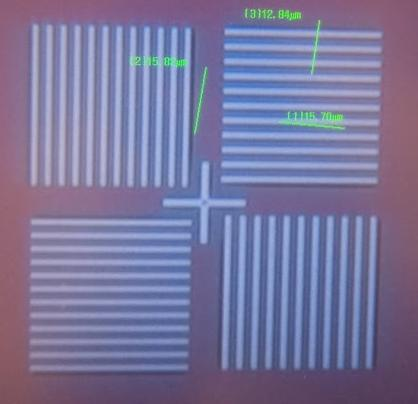
\includegraphics[scale=0.5]{pictures/alignment_cross.png}
	\caption{Picture of an alignment mark}
	\label{alignment_mark_target}
\end{figure}

How such an alignment mark might look like is being shown in \autoref{alignment_mark_target}, which is the ASML mark used for the ASML stepper units.

Depending on the alignment strategy there can be two or more alignment marks being etched into the substrate, and the positioning entirerly depends on
the pattern recognition software and alignment strategy of the specific machine.

The depth of this silicon etching is usually around 200nm or so, but is nothing really critical to support LibreSilicon but more something stepper
aligner specific.

The manufacturer of the stepper aligner usually provides pre made masks for this step and provide requirements for the depth of those marks inside the
silicon.

The ASML stepper has two alignment marks left and right of the wafer, which, when connected to a line, are in parallel to the notch.

Those marks are critical for aligning the patterns correctly above each other during all the further manufacturing steps, so it should be taken care,
that those markers stay always visible, so that the machine can find them and orient itself on it.

\newpage
\section{Shallow trench isolation}\label{sti_chapter}
The geometry of a substrate with STI implemented can be seen in \autoref{sti_target}.

\begin{figure}[H]
	\centering
	\begin{tikzpicture}[node distance = 3cm, auto, thick,scale=\CrossAndTopSectionBig, every node/.style={transform shape}]
		\input{tikz_process_steps/sti.a.tex}
	\end{tikzpicture}
	\begin{tikzpicture}[node distance = 3cm, auto, thick,scale=\CrossAndTopSectionBig, every node/.style={transform shape}]
		\input{tikz_process_steps/sti.b.tex}
	\end{tikzpicture}
	\caption{Shallow trench isolation target geometry}
	\label{sti_target}
\end{figure}

As can be seen in \autoref{tripple_well_target}, the STI trench is supposed to have approximately half the depth of the N-well.

Because the N-well will be $\approx 4 \mu m$ in depth, so we have to match this with our trench depth.

I order to allow a sufficiently low resistance of the ESD diode but at the same time a sufficient isolation of between the standard cells a trade-off has been done.

The targeted depth of the box isolation is $\approx 2 \mu m$.

The STI area will be everywhere, where no well areas are.

We use a dry etching method for cutting into the silicon substrate and making the active area become islands with trenches in between.

After that we fill the trenches with LTO and polish the wafer until the LTO surface and the silicon island surface are sufficiently on the same level.

Our minimum width and height as well as the space between the active areas comes from the line space constrain of the silicon etcher and of course the optical limitations of the stepper which are as well 0.5\um.

\newpage

\subsection{CMP end stop}\label{sti_end_stop}

In order to prevent irreversible damage to the crystal lattice of the active area, we need to provide a CMP end stop on top of those areas.

\begin{figure}[H]
	\centering
	\begin{tikzpicture}[node distance = 3cm, auto, thick,scale=\CrossSectionOnly, every node/.style={transform shape}]
		\input{tikz_process_steps/sti.end_stop.a.tex}
	\end{tikzpicture}
	\drawStepArrow{}
	\begin{tikzpicture}[node distance = 3cm, auto, thick,scale=\CrossSectionOnly, every node/.style={transform shape}]
		\input{tikz_process_steps/sti.end_stop.b.tex}
	\end{tikzpicture}
	\caption{End stop}
\end{figure}

The wafer is cleaned by being put into sulfuric acid at 120\degreesC and afterwards HF dipped in order to remove the native oxide.
After that a more uniform and very thin film of thermal oxide is being grown, the thickness can be around 10nm, this can be achieved by putting the wafer into a furnace at 1000\degreesC for 15 minutes in an $O_2$ environment (dry oxidation).
On top of this pad oxide, a layer of around 100nm of nitride is being deposited, using chemical vapor deposition.

\subsection{Silicon etching}\label{sti_trench_etch}

The trench depth has to be at least 2 microns and less than 4 microns deep, in order to have a sufficiently good isolation for preventing latchup effects and at the same time still good enough ESD diode behaviour.

\begin{figure}[H]
	\centering
	\begin{tikzpicture}[node distance = 3cm, auto, thick,scale=\CrossSectionOnly, every node/.style={transform shape}]
		\input{tikz_process_steps/sti.silicon_etch.a.tex}
	\end{tikzpicture}
	\drawStepArrow{}
	\begin{tikzpicture}[node distance = 3cm, auto, thick,scale=\CrossSectionOnly, every node/.style={transform shape}]
		\input{tikz_process_steps/sti.silicon_etch.b.tex}
	\end{tikzpicture}
	\caption{Trench etching}
\end{figure}

After patterning the STI layout the resist is being hard baked and the nitride+pad oxide is being etched, using plasma etching for nitride+oxide.

After etching the nitride and oxide we use a DRIE etcher and set the number of cycles in a way that it results in around 2 microns trench depth.

Adding to the over etch from the previous etch step, this will result in a depth a little bit deeper than 2 microns.

\newpage

\subsection{Liner oxide}\label{sti_liner_oxide}

In order to improve the interface properties of the LTO deposited in \autoref{sti_lto_deposition} to the side walls of the silicon islands a thin layer of thermal oxide is being grown after DRIE etching.

\begin{figure}[H]
	\centering
	\begin{tikzpicture}[node distance = 3cm, auto, thick,scale=\CrossSectionOnly, every node/.style={transform shape}]
		\input{tikz_process_steps/sti.liner_oxide.a.tex}
	\end{tikzpicture}
	\drawStepArrow{}
	\begin{tikzpicture}[node distance = 3cm, auto, thick,scale=\CrossSectionOnly, every node/.style={transform shape}]
		\input{tikz_process_steps/sti.liner_oxide.b.tex}
	\end{tikzpicture}
	\caption{Liner oxide}
\end{figure}

The interface oxide, as the pad oxide, only has to be a few nanometers in thickness, this can be achieved by putting the wafer again into a furnace at 1000\degreesC for 15 minutes in an $O_2$ environment (dry oxidation).

\subsection{LTO deposition}\label{sti_lto_deposition}

Now we fill up the trenches we've etched before with LTO for further planarization in \autoref{sti_cmp_step}

\begin{figure}[H]
	\centering
	\begin{tikzpicture}[node distance = 3cm, auto, thick,scale=\CrossSectionOnly, every node/.style={transform shape}]
		\input{tikz_process_steps/sti.lto.a.tex}
	\end{tikzpicture}
	\drawStepArrow{CVD}
	\begin{tikzpicture}[node distance = 3cm, auto, thick,scale=\CrossSectionOnly, every node/.style={transform shape}]
		\input{tikz_process_steps/sti.lto.b.tex}
	\end{tikzpicture}
	\caption{Oxide deposition}
\end{figure}

The easiest method is to put the wafer into a CVD furnace in order to deposit around 2 microns of LTO.

Better uniformity of the LTO film can be achieved by getting the boat out after every deposited 500nm, rotating it 90 degrees and putting it back in for another deposition round.

Also remember to measure the thickness of the deposited LTO under a spectroscope, in order to calculate the approximate CMP time!

\newpage

\subsection{CMP step}\label{sti_cmp_step}

Now the LTO needs to be planarized until a sufficiently low height differential between the oxide surface and the silicon surface is being met.

\begin{figure}[H]
	\centering
	\begin{tikzpicture}[node distance = 3cm, auto, thick,scale=\CrossSectionOnly, every node/.style={transform shape}]
		\input{tikz_process_steps/sti.cmp.a.tex}
	\end{tikzpicture}
	\drawStepArrow{CMP}
	\begin{tikzpicture}[node distance = 3cm, auto, thick,scale=\CrossSectionOnly, every node/.style={transform shape}]
		% substrate
\fill[isolationoxide] (0,0) rectangle (55,\STIIslandSurface);

\newcommand{\leftslope}[1]{
\filldraw[line width=0, isolationoxide] (#1-1.0,\STIIslandSurface) -- (#1,\STIIslandSurface) -- (#1,\STIIslandSurface+1.0);
}
\newcommand{\rightslope}[1]{
\filldraw[line width=0, isolationoxide] (#1,\STIIslandSurface) -- (#1+1.0,\STIIslandSurface) -- (#1,\STIIslandSurface+1.0);
}

\leftslope{1.25}
\leftslope{9.75}
\leftslope{18.25}
\leftslope{26.75}
\leftslope{35.25}

\rightslope{8.25}
\rightslope{16.75}
\rightslope{25.25}
\rightslope{33.75}
\rightslope{42.25}

\input{tikz_process_steps/sti.liner_oxide.a.tex}

\fill[isolationoxide] ( 1.25,\STIIslandSurface)      rectangle ( 8.25,\STIIslandSurface+0.25);
\fill[nitride]        ( 1.25,\STIIslandSurface+0.25) rectangle ( 8.25,\STIIslandSurface+1.0);

\fill[isolationoxide] ( 9.75,\STIIslandSurface)      rectangle (16.75,\STIIslandSurface+0.25);
\fill[nitride]        ( 9.75,\STIIslandSurface+0.25) rectangle (16.75,\STIIslandSurface+1.0);

\fill[isolationoxide] (18.25,\STIIslandSurface)      rectangle (25.25,\STIIslandSurface+0.25);
\fill[nitride]        (18.25,\STIIslandSurface+0.25) rectangle (25.25,\STIIslandSurface+1.0);

\fill[isolationoxide] (26.75,\STIIslandSurface)      rectangle (33.75,\STIIslandSurface+0.25);
\fill[nitride]        (26.75,\STIIslandSurface+0.25) rectangle (33.75,\STIIslandSurface+1.0);

\fill[isolationoxide] (35.25,\STIIslandSurface)      rectangle (42.25,\STIIslandSurface+0.25);
\fill[nitride]        (35.25,\STIIslandSurface+0.25) rectangle (42.25,\STIIslandSurface+1.0);

\draw[<->] (42.25,\STIIslandSurface+1.0) -- (42.25,\STIIslandSurface);
\node at (42.5,\STIIslandSurface+0.5) {$\Delta h$};


	\end{tikzpicture}
	\drawStepArrow{Nitride strip}
	\begin{tikzpicture}[node distance = 3cm, auto, thick,scale=\CrossSectionOnly, every node/.style={transform shape}]
		\input{tikz_process_steps/sti.cmp.c.tex}
	\end{tikzpicture}
	\caption{After CMP}
\end{figure}

A CMP is performed, based on a rough time calculation, based on the thickness measurement from \autoref{sti_lto_deposition}, until a height differential (See $\Delta h$ in graphics) below 200nm is being reached, which can be determined by using a surface profiler.

If available the slurry "SRS-985" should be used because it can significantly increase the yield by reducing the dishing as a study has found\footnote{\url{https://download.libresilicon.com/papers/10.1.1.567.8814.pdf}}.

After the planarization the wafer needs to be cleaned in hot ammonia and with RCA solution and wafers should kept wet in DI water after CMPing and should not dry out before being cleaned, because this would make particles get stuck in the oxide permanently and will destroy the sample.

After cleaning the LTO has to be annealed in order to increase the etching time when removing the pad oxide: The sample is being put into a furnace for 30 minutes at 850\degreesC in an inert atmosphere ($N_2$/$Ar$).

The densification is being performed before nitride strip, because the Phosphoric acid also attacks oxide, and by hardening the LTO first, we can reduce the amount of oxide, which is being removed alongside the nitride.

After the annealing the nitride is first stripped in a suitable nitride etchant like Phosphoric acid or the like.

After that the pad oxide beneath is being removed by being put into BOE for a few minutes until the pad oxide has been removed.

In this process, the sharp corners of the craters in the oxide, where the nitride used to be will also be smothened out, which is a nice side effect.


\newpage
\input{process_hightech_tripple_well.tex}
\newpage
\input{process_hightech_fox.tex}
\newpage
\input{process_hightech_sonos.tex}
\newpage
\input{process_hightech_gate.tex}
\newpage
\input{process_hightech_junctions.tex}
\newpage
\section{Silicification}\label{step_silicification}

Titanium silicide is one of the first SALICIDE material introduced in ULSI devices owing to its low resistivity, high thermal stability, ease in deposition and compatibility with silicon processes.
Titanium has been one of the familiar materials in ULSI productions, which is also an important advantage in practical use of titanium SALICIDE.\footnote{A Study on Formation of High Resistivity Phases of Nickel Silicide at Small Area and its Solution for Scaled CMOS Devices, 07D53437, Ryuji Tomita}

\begin{figure}[H]
	\centering
	\begin{tikzpicture}[node distance = 3cm, auto, thick,scale=\CrossAndTopSectionBig, every node/.style={transform shape}]
		\fill[isolationoxide] (0,0) rectangle (55.0,\LowerMetal);

\paintactivecover{nitride}{0.5}
\paintactivecover{isolationoxide}{0.25}

\filldraw[line width=0, nitride] (5.00,\STIIslandSurface) -- (4.50,\STIIslandSurface) -- (5.00,\STIIslandSurface+1.4);
\filldraw[line width=0, nitride] (6.00,\STIIslandSurface) -- (6.50,\STIIslandSurface) -- (6.00,\STIIslandSurface+1.4);

\filldraw[line width=0, nitride] (12.00,\STIIslandSurface) -- (11.50,\STIIslandSurface) -- (12.00,\STIIslandSurface+1.4);
\filldraw[line width=0, nitride] (13.50,\STIIslandSurface) -- (13.00,\STIIslandSurface) -- (13.00,\STIIslandSurface+1.4);

\filldraw[line width=0, nitride] (21.40,\STIIslandSurface) -- (21.90,\STIIslandSurface) -- (21.90,\STIIslandSurface+1.6);
\filldraw[line width=0, nitride] (22.90,\STIIslandSurface) -- (23.40,\STIIslandSurface) -- (22.90,\STIIslandSurface+1.6);

\fill[nitride] (44.0,\polytop+0.75) rectangle (44.8,\polytop+1.25);
\fill[nitride] (44.5,\polytop+0.75) rectangle (46.5,\implantstoptop+0.5);
\fill[nitride] (46.2,\polytop+0.75) rectangle (47.0,\polytop+1.25);

\fill[nitride] (49.5,\polytop+0.75) rectangle (53.5,\polytop+1.25);

\input{tikz_process_steps/pimplant.a.tex}

\fill[silicide] ( 1.35,\STIIslandSurface-0.1) rectangle ( 2.35,\STIIslandSurface);
\fill[silicide] ( 2.70,\STIIslandSurface-0.1) rectangle ( 4.50,\STIIslandSurface);
\fill[silicide] ( 5.00,\STIIslandSurface+1.3) rectangle ( 6.00,\STIIslandSurface+1.4);
\fill[silicide] ( 6.50,\STIIslandSurface-0.1) rectangle ( 8.15,\STIIslandSurface);

\fill[silicide] ( 9.85,\STIIslandSurface-0.1) rectangle (11.50,\STIIslandSurface);
\fill[silicide] (12.00,\STIIslandSurface+1.3) rectangle (13.00,\STIIslandSurface+1.4);
\fill[silicide] (13.50,\STIIslandSurface-0.1) rectangle (15.25,\STIIslandSurface);
\fill[silicide] (15.60,\STIIslandSurface-0.1) rectangle (16.60,\STIIslandSurface);

\fill[silicide] (19.20,\STIIslandSurface-0.1) rectangle (20.20,\STIIslandSurface);
\fill[silicide] (20.60,\STIIslandSurface-0.1) rectangle (21.40,\STIIslandSurface);
\fill[silicide] (21.90,\STIIslandSurface+1.5) rectangle (22.90,\STIIslandSurface+1.6);
\fill[silicide] (23.40,\STIIslandSurface-0.1) rectangle (24.20,\STIIslandSurface);

\fill[silicide] (26.90,\STIIslandSurface-0.1) rectangle (27.90,\STIIslandSurface);
\fill[silicide] (28.35,\STIIslandSurface-0.1) rectangle (29.35,\STIIslandSurface);
\fill[silicide] (29.80,\STIIslandSurface-0.1) rectangle (30.80,\STIIslandSurface);
\fill[silicide] (31.25,\STIIslandSurface-0.1) rectangle (32.15,\STIIslandSurface);
\fill[silicide] (32.60,\STIIslandSurface-0.1) rectangle (33.60,\STIIslandSurface);

\fill[silicide] (35.60,\STIIslandSurface-0.1) rectangle (36.50,\STIIslandSurface);
\fill[silicide] (36.95,\STIIslandSurface-0.1) rectangle (37.85,\STIIslandSurface);
\fill[silicide] (38.30,\STIIslandSurface-0.1) rectangle (39.20,\STIIslandSurface);
\fill[silicide] (39.65,\STIIslandSurface-0.1) rectangle (40.55,\STIIslandSurface);
\fill[silicide] (41.00,\STIIslandSurface-0.1) rectangle (41.90,\STIIslandSurface);

% diode contacts
\fill[silicide] (43.00,\STIIslandSurface+2.0) rectangle (44.00,\STIIslandSurface+2.15);
\fill[silicide] (47.00,\STIIslandSurface+2.0) rectangle (48.00,\STIIslandSurface+2.15);

% resistor contacts
\fill[silicide] (48.50,\STIIslandSurface+2.0) rectangle (49.50,\STIIslandSurface+2.15);
\fill[silicide] (53.50,\STIIslandSurface+2.0) rectangle (54.50,\STIIslandSurface+2.15);



	\end{tikzpicture}
	\caption{Silicide geometry target}
	\label{policide_silicide_sections}
\end{figure}

In order to reduce the gate contact resistance as well as the source and drain resistance and in order to provide a more effective etch stop when plasma etching the contact windows to drain, source and gate, silicide/polycide is being added to the wafer as shown in \autoref{policide_silicide_sections}.

The side walls\footnote{\url{http://www.fujitsu.com/jp/group/mifs/en/resources/news/library/tech-intro/process/side-wall.html}} are required in order avoid short circuits between the junction and the gate.

When titanium and silicon are brought into contact and heated at temperatures above 800 \degree C (in the presence of excess silicon) $Ti Si_2$ forms.

The $TiSi_2$ has a resistivity of $12-20 \mu\Omega - cm$.

The basic formation process of titanium SALICIDE is as follows:

A thin titanium film of roughly 30 nm thickness is deposited on an entire wafer with MOSFETs structure.

The deposited Ti film reacts with the exposed silicon areas such as the source/drain area and polysilicon gate electrodes during the annealing at 800\degree C in Argon atmosphere.

Then, the unreacted titanium film on the dielectric layer such as $SiO_2$ or SiN is selectively etched by RCA-1 (Ammonia and Hydrogen Peroxide Mixture) solution for around 2-3 minutes.

\newpage

\subsection{Nitride deposition}\label{nitride_spacers_deposition}

The thickness of this CVD deposited nitride layer will be the width of the spacer after having used highly anisotropic etching in the next few steps, for this reason the thickness of the nitride decides over the distance between the silicide and the gate oxide.

Considering, due to the edge effects during dry etching, the thickness of the nitride has to be less than 25\% of the polysilicon thickness, we choose 50nm for the nitride thickness.

\begin{figure}[H]
	\centering
	\begin{tikzpicture}[node distance = 3cm, auto, thick,scale=\CrossSectionOnly, every node/.style={transform shape}]
		\input{tikz_process_steps/silicification.nitride_deposition.a.tex}
	\end{tikzpicture}
	\drawStepArrow{Nitride CVD}
	\begin{tikzpicture}[node distance = 3cm, auto, thick,scale=\CrossSectionOnly, every node/.style={transform shape}]
		\input{tikz_process_steps/silicification.nitride_deposition.b.tex}
	\end{tikzpicture}
	\caption{Nitride layer}
\end{figure}

The deposition rates might variate between LPCVDs and recipes. It's at the discretion of the operation engineer to achieve those 50nm.

\subsection{Spacer etching}

Now we have to etch our nitride as anisotropic as possible.

This means that the etching mostly only comes "from above" with a few to nearly none horizontal etching.

Thit means the etching process only "sees" the sidewall as a "thicker layer" and starts etching downward.

\begin{figure}[H]
	\centering
	\begin{tikzpicture}[node distance = 3cm, auto, thick,scale=\CrossSectionOnly, every node/.style={transform shape}]
		\input{tikz_process_steps/silicification.sputter_etching.a.tex}
	\end{tikzpicture}
	\drawStepArrow{Dry etching}
	\begin{tikzpicture}[node distance = 3cm, auto, thick,scale=\CrossSectionOnly, every node/.style={transform shape}]
		\input{tikz_process_steps/silicification.sputter_etching.b.tex}
	\end{tikzpicture}
	\caption{Anisotropic etching}
\end{figure}

After that we will have our desired spacer geometry forming as well as any potentially resist covered area from the silicide block mask patterns, which will allow us to control in which areas we reduce the sheet resistance in which we don't.

\newpage

\subsection{Titanium deposition}

We deposit a layer of titanium with a thickness of between 30nm to 50nm which will then be reacted into titanium-silicide and titanium-polycide respectively in the further steps.

\begin{figure}[H]
	\centering
	\begin{tikzpicture}[node distance = 3cm, auto, thick,scale=\CrossSectionOnly, every node/.style={transform shape}]
		\input{tikz_process_steps/silicification.metal_deposition.a.tex}
	\end{tikzpicture}
	\drawStepArrow{Sputtering}
	\begin{tikzpicture}[node distance = 3cm, auto, thick,scale=\CrossSectionOnly, every node/.style={transform shape}]
		\input{tikz_process_steps/silicification.metal_deposition.b.tex}
	\end{tikzpicture}
	\caption{Titanium deposition}
\end{figure}

The titanium can either be applied by sputtering or by chemical deposition.

Depending on the technique of sputtering or deposition, the capabilities to deposit only 30nm may not be given.

It should however be avoided to deposit too much titanium (more than 100nm or so), because the etch rate of RCA-1 at room temperature
has a very good selectivity towards titanium compared to $Ti Si_2$ but is not 100\% perfect, which might lead to partial etching of
the $Ti Si_2$ film which might negatively impact the sheet resistance properties of the devices.

\subsection{Silicide formation}

The deposited Ti film reacts with the exposed silicon areas such as the source/drain area and polysilicon gate electrodes during RTP (Rapid Thermal Processing) at 800\degreesC in Argon ambient for 30 seconds.

In this annealing step the $Ti Si_2$ is formed.

\begin{figure}[H]
	\centering
	\begin{tikzpicture}[node distance = 3cm, auto, thick,scale=\CrossSectionOnly, every node/.style={transform shape}]
		\input{tikz_process_steps/silicification.rtp1.a.tex}
	\end{tikzpicture}
	\drawStepArrow{RTP}
	\begin{tikzpicture}[node distance = 3cm, auto, thick,scale=\CrossSectionOnly, every node/.style={transform shape}]
		\input{tikz_process_steps/silicification.rtp1.b.tex}
	\end{tikzpicture}
	\caption{RTP treatment}
\end{figure}

The resulting $Ti Si_2$ film will be around 77nm in tickness with around 20nm unreacted titanium left on top.

A color change into a slightly brownish color from originally silver metallic can be observed of the titanium on top of the oxide.

\newpage

\subsection{Metal removal}

The unreacted titanium film on the dielectric layer such as $SiO_2$ or $SiN$ is selectively etched by RCA-1 (Ammonia and Hydrogen Peroxide Mixture) solution.

\begin{figure}[H]
	\centering
	\begin{tikzpicture}[node distance = 3cm, auto, thick,scale=\CrossSectionOnly, every node/.style={transform shape}]
		\input{tikz_process_steps/silicification.metal_removal.a.tex}
	\end{tikzpicture}
	\drawStepArrow{RCA cleaning}
	\begin{tikzpicture}[node distance = 3cm, auto, thick,scale=\CrossSectionOnly, every node/.style={transform shape}]
		\input{tikz_process_steps/silicification.metal_removal.b.tex}
	\end{tikzpicture}
	\caption{Titanium etch}
\end{figure}

After 2-3 minutes in RCA-1, at room temperature, with a bit mechanical help, all the unreacted Titanium should be gone and the oxide should become visible again.
Under \textbf{no circumstance} use a solvent containing HF, since $Ti Si_2$ dissolves in HF or any other Fluoride containing solutions.

Better cleaning results can be achieved by adding mechanical stress to the unreacted metal while having it inside the RCA-1 solution,
so if you can put it into an ultrasonic bath, the RCA-1 cleaning results can be improved by this.

\newpage

\subsection{CMP}\label{chapter_silicide_and_cmp}

After we formed all the active devices and added the silicide in order to reduce the sheet resistance of junctions and contacts we have to make sure that
our devices will not be damaged during the planarization phase in order to contact through to them with the first metal layer.

\begin{figure}[H]
	\centering
	\begin{tikzpicture}[node distance = 3cm, auto, thick,scale=\CrossSectionOnly, every node/.style={transform shape}]
		\input{tikz_process_steps/silicification.cmp_stop.a.tex}
	\end{tikzpicture}
	\drawStepArrow{LTO+CMP}
	\begin{tikzpicture}[node distance = 3cm, auto, thick,scale=\CrossSectionOnly, every node/.style={transform shape}]
		\input{tikz_process_steps/silicification.cmp_stop.b.tex}
	\end{tikzpicture}
	\caption{CMP, contact preparation}
\end{figure}

First we deposit around 100nm LTO as a pad oxide layer below the 100nm nitride, which serves as the CMP stop hard mask.
Then we deposit 1\um LTO and CMP away the height differential of the active devices translated to the oxide.

LTO was chosen because the silicide becomes unstable in the thermal ranges where phosphorus silicate glass becomes viscous enough
for evening out the height differential by evening out by seeking its level during annealing.

A thickness of 1\um of the LTO will make it less likely, that the dishing effect of the CMP pad causes devices to get damaged
through an over consumption of the nitride hard mask.

The best approach for depositing this LTO layer is to split the deposition into 4 steps at each 250nm and rotating the sample
90 degrees between the steps in order to improve uniformity of the LTO layer.

\newpage
\input{process_hightech_interconnect.tex}

\end{document}
